% Resultados
\chapter{Implementaci\'on y Resultados} \label{chap:impresultados}

%Puedes quitar esto(es opcional)
\vspace{5 mm}

\section{Lenguaje usado}  \label{sec:lusado}

El proyecto fue hecho usando C++. Se elegi\'o \'este debido 
a su eficiencia, ya que compila a c\'odigo de m\'aquina y permite una buena
abstraci\'on de los problemas con las clases. Adem\'as, su librer\'ia ya contiene bastantes
cosas ya hechas, por lo que va a ahorrar tiempo de programaci\'on.

El dise\~no de las clases es el siguiente:

\begin{figure}[htb]
\centering
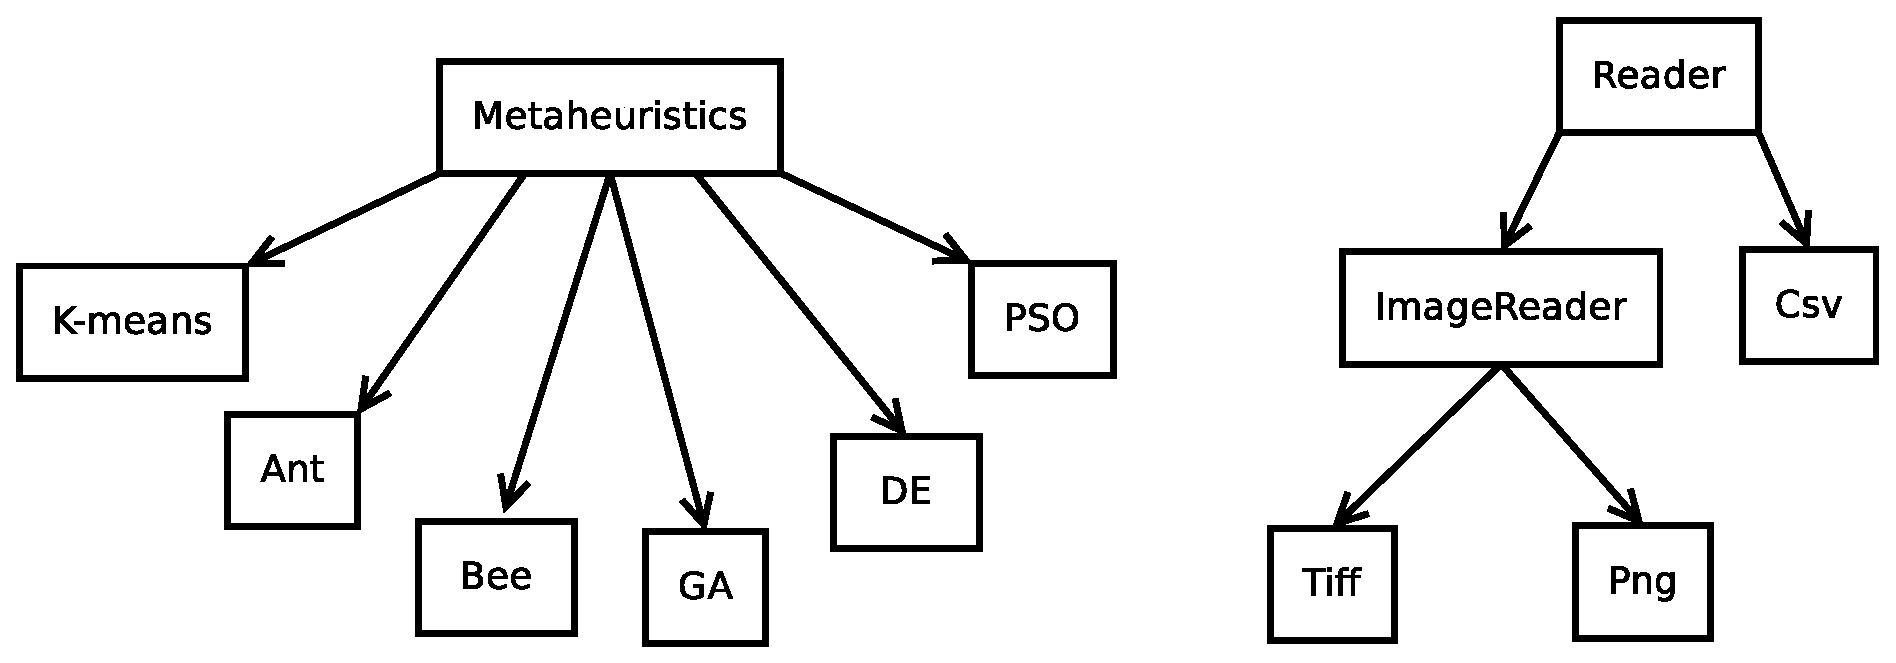
\includegraphics[scale=0.35]{figures/clases.eps}
\caption{Dise\~no de clases}
\label{fig:jclases}
\end{figure}

Donde Metaheuristics es una clase abstracta, que posee las m\'etodos que seran
usados por las diversas metaheur\'isticas hijas. En especial tienen dos 
importantes: initialize y run. El primero se va a encargar de inicializar el algoritmo
para que luego sea ejecutado. Por ejemplo en el gen\'etico inicializa aleatoriamente
las soluciones. Y el run es en s\'i el que va a ejecutar el algoritmo haciendo 
uso de los par\'ametros y variables ya inicilizadas.

Por el otro lado Reader tambi\'en
es una clase abstracta y es la que se encarga de definir lo m\'etodos que van a 
tener sus descendientes a la hora de leer un archivo, que se implement\'o para 
tres tipos: csv, png y tiff.

\section{M'aquina de prueba} \label{sect:testbed}

Todas las pruebas fueron realizadas con el computador cuyas caracter'isticas
aparecen en el cuadro \ref{tb:testbed}. La herramienta {\tt mhs} fue
compilada sobre esa m'aquina, exclusivamente con optimizaci'on gcc de nivel 3,
que es el nivel m\'as alto que posee gcc y aplica todas las mejoras
que este posee.

\begin{table}[htb]
\footnotesize
\begin{center}
\begin{tabular}{|>{\columncolor{lightgray}}c|c|}
\hline
CPU & Intel Core I5 650 \\
\hline
RAM & 6 GB \\
\hline
Distribuci'on & Ubuntu 11.04 x86\_64 bits \\
\hline
Kernel Linux & 2.6.38-8-generic \\
\hline
Versi'on gcc & 4.5.2 \\
\hline
\end{tabular}
\caption{Computador usado para las pruebas}
\label{tb:testbed}
\end{center}
\end{table}

\section{M\'etricas usadas}  \label{chap:meusada}

Para medir la distancia entre dos patrones se va a usar la euclidiana que
ya fue explicada en \ref{sect:mdist}. Se elegi\'o esta debido
a su f\'acil implementaci\'on, buenos resultado y rapidez.

La funci\'on objetivo principal es la DB, comentada en \ref{sect:tval}.
Su baja complejidad algor\'itmitca en comparaci\'on con las dem\'as existentes y
su eficacia en medir bien las dos cosas que se buscan en los cluster (distancia
intracluster baja e intercluster alta) fueron los motivos para su elecci\'on. 

El DE y PSO usan la propuesta por \cite{OmEnSa2005}. En el contexto de 
clustering de datos, una partícula o indivuduo representa
al centroide de un cluster. La calidad
de cada uno es medida usando:

\[
f(x_i,Z_i) = w_1 \overline{d}_{Max}(Z_i,x_i) + w_2 (z_{Max} - d_{Min}(x_i)) + w_3 J_{e,i}
\]

donde $z_{Max}$ es el máximo valor del conjunto de datos (en el contexto
de imágenes digitales $z_{Max} = 2^s - 1$ para una imagen de $s$-bits);
$Z_i$ es la matriz representando la asignación de patrones a los clusters
de la partícula $i$. Las constantes $w_1$, $w_2$ y $w_3$ son definidas por el usuario
usadas para determinar la contribución de cada uno de los sub-objetivos.
También

\[
\overline{d}_{Max}(Z_i,x_i) = \max_{1 \leq k \leq K} \left[ \displaystyle\sum_{\forall z_p \in C_{i,k}} d(z_p,m_{i,k})/n_{i,k}\right]
\]

es la máxima distancia eucl\'idea promedio de las partículas en sus
clusters asociados. Y

\[
\overline{d}_{Min}(x_i) = \min_{\forall k, l, k \neq l} \left[ d(m_{i,k},m_{i,l})\right]
\]

es la distancia eucl\'idea mínima entre un par de clusters.

Por \'ultimo $J_e$ es la comentado en \ref{sect:tval}.

Para comparar que tan bueno es un algoritmo en comparacaci\'on a los otros, todos son evaluados al final con $DB(K)$ 
y la del error $J_e$.

\section{Ajuste de par\'ametros}  \label{chap:ajustep}

Para cada metaheut\'istica hay que ver la influencia que sus par\'ametros 
poseen, buscar los m\'as adecuados y dar los resultados obtenidos.
Para ellos los pruebas se har\'an en dos pasos:

\begin{enumerate}

\item Hacer pruebas con todas las metaheur\'isticas variando los par\'ametros 
en todo su rango. Algunos par\'amtros como el n\'umero de iteraciones se mantiene
en un valor fijo que proviene de hacer pruebas emp\'iricas.

\item Con estos resultados, hacer un an\'alisis ANOVA para ver la influencia de cada
uno y de esta forma crear otras pruebas mucho m\'as espec\'ificas.

\end{enumerate}

\section{K-means}  \label{chap:ikmeans}

\'Este fue implementado tal cual como se explic\'o en \ref{sect:cpart}. La
inicializaci\'on es totalmente aleatoria. Y la condici\'on de paradas
va a ser hasta que no se mejores un n\'umero de veces dado.

\section{Bee}  \label{chap:ibee}

\section{Gen\'etico}  \label{chap:igenetico}

Se leyeron todas las posbibles formas propuestas por \cite{HrCaFr2009} y se decidi\'o
lo siguiente:

\begin{itemize}

\item Los cromosomas van a ser los centroides de los clusters, de un tama\~no de $K$
dado. Esto permite que las operaciones que se hagan sobre los individuos tengan
un efecto mas fuerte sobre el cluster y trabajen de manera mas global: sobre cluster y
no con objetos.

\item La mutaci\'on no es exclusiva de los hijos como se propuso en el marco te\'orico,
sino que es a cualquier miembro de la poblaci\'on. Son tres posibles: dividir un cluster
en dos, creando uno nuevo, unir dos cluster, y cambiar un elemento de un cluster a otro.
De esta forma hay una buena variedad y buenos cambios que pueden lograr obtener buenos
resultados.

\item La selecci\'on es por torneo, donde al comienzo del algoritmo se especifica 
el tama\~no de \'esta.

\item La condici\'on de parada es un n\'umero dado de veces que no se mejore lo 
que se tiene.

\item El resto del algoritmo sigue tal cual como ya se explic\'o.

\end{itemize}

\section{DE}  \label{chap:ide}

Se bas\'o en los trabajos hecho por \cite{SwAjAm2008} y \cite{OmEnSa2005}, especialmente
de \'este \'ultimo.

Se requiere un $K$ de antemano y los individuos van a ser arreglos de $K$ centroides.
El algoritmo funciona tal cual como se explic\'o en \ref{sect:metade}. Una de las diferencias es
el cruce, donde adicionalemente se tiene
un punto entre $[1,M|$ donde es 100\% de probabilidad de cruce. La condici\'on
de parada es un n\'umero de iteraciones dado. Con respecto
a los par\'ametros $F$ y $Cr$, pueden ser establecidos o funcionar como se propone
en el primer art\'iculo, con ciertas modificaciones:

\begin{itemize}

\item {\bf $F$:} En cada iteraci\'on se calcula un nuevo $F$, con la siguiente expresi\'on:
$0.5 \times (1 + rand(0,1))$, donde $rand(0,1)$ es un n\'umero aletorio entre $[0,1]$.
Es claro que la media va a ser 0.75. \'Esto permite variaciones estoc\'asticas en el vector diferencia, y
por lo tando ayuda a mantener diversa la poblaci\'on a medida que la b\'usqueda progresa.

\item {\bf $Cr$:} Se establece un $Cr_{max}$ y $Cr_{min}$. La idea es que el $Cr$ vaya
decrementando linealmente desde el primero hasta el segundo. Al comienzo
se desea que explorar el espacio de b\'usqueda y al final se enfoquarse y mejorar las soluciones
que ya se llevan. Es f\'acil ver a medida que el $Cr$ disminuye, los hijos heradan m\'as
del padre. Se tomaron $Cr_{max} = 1.0$ y $Cr_{min} = 0.5$. La variaci\'on esta expresada por:

\[
(Cr_{max}-Cr_{min}) \times {{maxit - it} \over maxit} + Cr_{min}
\]

donde $maxit$ es el n\'umero de iteraciones tope dado al algoritmo e $it$ es la iteraci\'on actual.

\end{itemize}

\section{PSO}  \label{chap:ipso}

\section{Hormiga}  \label{chap:ihormiga}

Como se mencion\'o en \ref{sect:metaant} hay varias visiones de esta metaheur\'istica.
La primera es la que se basa en la b\'usqueda de comida por parte de las hormigas.
\'Esta es inviable para hacer clustering porque no se puede representar 
una soluci\'on mediante un grafo. Por ello es usada la otra perspectiva basada en c\'omo
las hormigas arman sus cementerios u organizan de las c\'rias. 

En \'esta las hormigas se van a mover en un grid de dos dimensiones. Si 
el tama\~no es muy peque\~no van a hacer muchos movimientos en vista que
no van a conseguir espacios vacios donde soltar el objeto que cargan. En cambio,
si es muy grande se haran movimientos innecesarios cuando la hormiga no lleva nada.
No hay una gu\'ia te\'orica del tama\~no adecuado. Por ello la implemetaci\'on que
se hizo fue basada de \cite{OuBa2007}, donde se propone usar un arreglo 
de $N/4$ c\'elulas en el cual las hormigas se pueden mover libremente.
Una de las ventajas es lo f\'acil de identificar los clusters a diferencia
de un grid donde no existe un modo establecido para lograrlo.

Al comienzo los $N$ patrones son colocados
en las c\'elulas de forma aleatoria. Luego se tienen $na$ hormigas que van a tomar
un pixel de forma aleatoria. Posterior comienza un ciclo donde se selecciona una hormiga
aleatoriamente. Si la hormiga no carga ning\'un pixel, est\'a busca un pixel
que no este siendo cargado por otra hormiga y probabilisticamente decide si agarrarlo o dejarlo.
En el caso contrario, busca una c\'elula donde soltar su pixel e igual que antes
probabil\'isticamente decide si soltarlo o quedarselo. Las hormigas van a poseer
una memoria global donde se guarda donde se han soltado los p\'ixeles.
De tal forma primero revisa en estos recuerdos e intenta dejarlo con el que tenga 
mayor probabilidad de hacerlo, sino simplemente trata en una c\'elula
aleatoria. Cada 100 iteraciones se va a eliminar de
el menos usado y de esta forma se va variando la memoria, y se mantienen los que
esten ayudando m\'as/. Otro aspecto es que cada cierto n\'umero de veces que
se intenta modificar la memoria, se le elimina el elemento que ha sido dejado en menos c\'elulas,
de esta forma se aumenta la diversidad y los mejores se mantienen.

Se tiene

\[
f(p_i,c_k) = {1 \over n_k} \sum_{p_j \in c_k} {\alpha^2 \over {\alpha^2 + d(p_i,p_j)^2}}
\]

donde $d_(p_i,p_j)$ es una funci\'on de disimilaridad
entres dos patrones y $\alpha$ es el promedio de todas
las diferencias entre los patrones:

\[
\alpha = {1 \over {N*(N-1)}} \sum_{j=1}^N \sum_{i=j+1}^N {2 \times d(p_i,p_j)}
\]

La probabilidad de agarrar un pixel es:

\[
p_{pick}(p_i,c_k) = 
\begin{cases}
1 & \text{si } |c_k| = 1 \\
q & \text{si } |c_k| = 2 \\
\cos( {\pi \over 2} f(p_i, c_k) )^2  & \text {sino}
\end{cases}
\]

Y la de soltarlo es:

\[
p_{drop}(p_i,c_k) = 1 - \cos( {\pi \over 2} f(p_i, c_k) )^2 
\]

El $q$ usado es el recomendado (0.7). Un psudoc\'odigo es
el siguiente:

\begin{lstlisting}[mathescape, language=Pascal]
  Inicialización.
  Hacer maxit veces
    Se toma una hormiga rn aleatoriamente
	Si rn tiene un pixel
	  Si la memoria no esta vacía
	    Buscar soltarlo en alguno de la memoria
		Sino lo dejo
		  Tratar de dejarlo en una célula aleatoria
	  Sino
	    Tratar de dejarlo en una célula aleatoria
	Sino
	  Tomar un pixel que no cargue ninguna hormiga de forma aleatoria
	  Tratar de tomarlo
  Reconstruir solución
\end{lstlisting}

El \'unico detalle que falta explicar es la parte de reconstruir la soluci\'on.
Primero lo que se hace es colocar en una c\'elula los pixeles
que no han soltado las hormigas. Luego se pasa de las c\'elulas al 
arreglo de soluci\'on usado por todas las metaheur\'isticas. Finalmente
se unen los clusters muy parecidos o que s\'olo tengan un elemento.


